\documentclass[12pt]{article}

% useful for formatting (align*, etc.) and for certain symbols (the QED box, etc.)
\usepackage{amsmath, amssymb, amsthm}

% for including graphics
\usepackage{graphicx}

% for conveniently specifying the spacing (\singlespacing, \doublespacing,
%    \onehalfspacing, etc.)
\usepackage{setspace}
\doublespacing

% this does some sort of symbol stuff
\usepackage{textcomp}

% A package for conveniently adjusting headers and such
\usepackage{fancyhdr}
\renewcommand{\headrulewidth}{0 pt}
\rhead{\textit{\thepage}}
\cfoot{}



% Set the margins
\usepackage[top=1.8cm, bottom=1.8cm, left=1.8cm, right=1.8cm]{geometry}
% set up a new command to insert a little bit of vertical space
% (use this BEFORE a line break)
\newcommand{\padding}{\vspace*{.5cm}}

% set up an environment to format each hw problem in
\newenvironment{problem}[1]{\noindent\textbf{#1.}}{\vspace*{.5cm}}

\newenvironment{proof*}{\par\noindent{\bf Proof}\quad}
               {\quad\vrule height 8pt depth 0pt width 8pt\medskip\par}



\begin{document}

%Add in some nice looking pages
 \begin{titlepage}
    \vspace*{\fill}
    \begin{center}
      {\Huge Vir-Pong: Android Development Team}\\[0.5cm]
      {\Large Jillian Andersen, Jordan Apele, David Ruhle, Kyle Wenholz}\\[0.4cm]
      \today
    \end{center}
    \vspace*{\fill}
  \end{titlepage}

\tableofcontents
\newpage
\section{Personnel Profile}

\subsection{Jordan Apele}
Jordan is a senior at University of Puget Sound pursuing a Bachelor of
Science in Computer Science/Business. She has taken both Computer Science 161
and 261, which are introductory into problem solving, and good programming style,
as well as fundamental data structures. She also has Database Designs experience
with the conceptual data modeling and query languages.

Jordan also has extensive leadership skills. While a Resident Assistant,
Jordan was able to gain experience with confrontation dissolution, community
building, and communication. She also interacted with about 30 residents as well
as a 10-member staff team. As the University of Puget Sound Kayak Club President,
Jordan gained experience coordinating a leadership board, management of pool
sessions, as well as acting as event management. Through her experience in Kayak Club,
Jordan learned how to both work as part of a team to bring everyone through safely
and was able to step up and take charge when it was needed.

Jordan also brings a driven work ethic and the ability to work independently
to the project. While working as an Administrative Assistant, Jordan was able to
manage her time independently to finish tasks assigned to her.

\vspace*{5mm}

\noindent \textbf{Technical Proficiencies}: Java, some HTML, Database Development, Eclipse, MySQL, BlueJ, familiarity with Windows and MacOS


\subsection{Jillian Andersen}
Jillian is a junior at the University of Puget Sound pursuing majors in Computer Science and Music
with an emphasis in Music History. As a result of her work ethic and personal experience, she has been very focused on clean project design. Several projects in her coursework required her to break apart large problems, generate a solution, and then thoroughly document said solution.  These strengths and experiences are
useful in a large-scale project such as the one we are undertaking.

Her experience in the music field has also prepared her for this project in unique ways.
Performing in front of others on a regular basis has helped to hone her presentation skills. She is
able to cope with the stress of public speaking, maintaining confidence and competence even when
nervous. Her experience of working in musical ensembles, has improved her ability to work
alongside a variety of personalities and egos; it has also strengthened her ability to work
effectively in a team to accomplish a common goal.

\vspace*{5mm}

\noindent \textbf{Technical Proficiencies}: Java, BlueJ, Eclipse, familiar with Windows, familiar with Microsoft Office


\subsection{Kyle Wenholz}
Kyle is a junior at University of Puget Sound, pursuing majors in Mathematics and Computer Science.  His background in Math makes him a strong addition to the theoretical aspects involved in our project: mapping out component relationships and determining functionality of various systems.  He also has a fair amount of experience working with programs through his coursework, but the most important part of his background is summer research.  Kyle's project focused on a psychological aspect of human-computer interaction, preparing him to ask difficult questions about the functionality and use of our software.  He has also dealt with open-ended issues and grappled with the many complexities of seeking answers where there may not yet be any.  Over the course of development, his strengths in theoretics will partner well with the talents of the other members on the Android development team.

\vspace*{5mm}

\noindent \textbf{Technical Proficiencies}: Java, Python, Git source control, Eclipse, familiarity with Linux and Windows

\subsection{David Ruhle}
\noindent David will receive a Bachelor of Science in Computer Science with a minor in Business from University of Puget Sound. He has taken computer science courses in programming languages, computer graphics,
Java development, operating systems, assembly language/computer architecture, and software
engineering. His courses in management, economics, personal finance, managerial finance, and marketing make him a valuable asset for creating a timely, accessible, and marketable product.

\vspace*{5mm}

\noindent \textbf{Technical Proficiencies}: Java, C, some C++, Prolog, Haskell, Eclipse, familiarity with Linux and Windows

\section{Proposed End Product}
Our end product will be a downloadable Android application for playing Pong.  The application takes position data from a Wii Remote and allows the user to move their paddle on screen with physical movement of their body.  The application is set up so that the user logs into the application with pre-registered information or as a guest and connects with other users.  At the end of a game the user either wins or looses, and may proceed to play another game or terminate the application.  The application can access user statistics, and global statistics, help and support all from the main menu.  Install instructions as well as help and support can be found on the Android market or on the Vir-Pong site. Developer documentation can be found on GitHub under the Vir-Pong organization.  The Android application will be integrated with the greater Vir-Pong system to create a service for playing games of human Pong, using the latest technology in human-computer interaction.

\section{Key Features}
There are a number of key features that must function properly in order for our program
to work on the most basic level. First, the Android device must be able to communicate with the
Wii Remote through Bluetooth, in order to acquire accelerometer data. This function is absolutely vital
because it allows the phone to track the position of the player and calculate the position of the
player's paddle. After gaining data from the Wii Remote, the phone needs to pass this information
along to a server. As the phone is sending position data, it must be able to also receive the
position of both players' paddles and ball location from the server. In addition, the application 
must receive information about when a point is scored, to whom the point goes to, when the game is over, and
the final score of the players. In order to allow players to see all of this data, there must be a
graphical representation of the game that is constantly updated by the server. Pairing down to
essentials, this would include only a plain background, two paddles, and a ball. This GUI must
also include a start screen that allows for players to choose to start a game and end the
application when the game is finished.  After the completion of these primary features, we can start working on secondary features that are not integral to the game, but enhance the playing experience. 

\subsection{Secondary Features}
The secondary features are extremely open-ended and allow for many creative possibilities.
\begin{itemize}
\item The ability to visit the Vir-Pong website on the Android browser ensures a seamless experience for users. 
\item The production sound effects or vibration effects on either the phone itself or on the Wii Remote may enhance player immersion.
\item The ability for users to change game settings, such as court size, ball speed and difficulty level. 
\item Allow the user to change graphic interface options, including pictures or logos to be used as the ball, color schemes, and game themes. 
\end{itemize}

\section{Tools for Development}
\begin{itemize}
\item Android SDK: The Android SDK acts as an emulator of an actual Android
phone, so that we can test our code as the project goes along, without
actually having to load up the phone every time. The Android SDK provides
the tools and APIs which allow us to develop applications for the Android
platform.  Download and install instructions can be found at 
\begin{verbatim}http://developer.android.com/sdk/index.html \end{verbatim}
\item Eclipse: Eclipse is a development environment which includes an integrated
development environment and a plug-in system. The plug-in system allows
us to add plug ins for the various programs like PhoneGap that we are using
for the application. Similarly Eclipse is multi-language so it works for most
of the coding we will be doing.  Download and install instructions can be found at 
\begin{verbatim}http://eclipse.org/downloads/ \end{verbatim}
\item JavaDocs: JavaDocs is a tool that generates documentation in HTML from
doc comments in source code. We will be using the library to reference
classes and packages to determine what methods or classes we will use.  These documents 
are generated from the source code and will be available with our final release on the 
web and, ideally, in the application.
\item Android Developers: Android Developers connects us with many resources
for programming on the Android, like SDK documentation and platform tools.  The link to 
this resource is
\begin{verbatim}
http://developer.android.com/index.html
\end{verbatim}
\item Themable Widget Library: Themable Widget Library is a library of GUI
components that we will be using for the project.  The library provides 
ease of access for us to create a better interface.  
Information on this library can be found at 
\begin{verbatim}
http://twl.l33tlabs.org/themeformat.html
\end{verbatim}
\item GitHub: GitHub is for sharing code between the groups of the project. It
is ideal for our software development project because we push our code
frequently into the repository and keep the project up to date for the teams
as a whole.  The source for the entire project is hosted under the following GitHub
organization:
\begin{verbatim}
https://github.com/organizations/VirPong/
\end{verbatim}
\item PhoneGap: PhoneGap is a mobile development framework that allows
programmers to build applications using JavaScript, HTML, and CSS. This
will be good for our project because it has the capability to be used on both an
Android and iPhone.  Information about this software can be found at
\begin{verbatim}
http://www.phonegap.com/
\end{verbatim}
\end{itemize}




\section{Challenges}

%Difficulties we face: streaming data between us and the server, creating a unified design, deploying to android 
% devices, 

Throughout our first few weeks we have planned such a great deal that our department feels confident in the development plan.  Despite the strength of this planning and the skills of our team, there will undoubtedly be challenges, many of which are certainly out of our control.  The challenges we anticipate going forward are outlined below: deploying to Android devices, communication with the server, and participating in a unified design.

\subsection{Deployment to Various Devices}
The Android OS runs on many devices, but this large hardware domain poses some difficulties.  These devices vary by processors, ports, interfaces, screen size, etc.  The differences in processor power will hopefully be a non-issue with clean and efficient code.  Ports and interfaces only limit our ability to expand into using peripherals aside from a Wii Remote.  The greatest of all these variances, however, is the screen size.  Our application must be developed for many aspect ratios and resolutions; moreover, the application must be playable on all of these.  Our use of HTML5 should help in avoiding issues here, with its support for tailoring sites to look appropriate on computers, handhelds, and various other devices.  The success of other companies in overcoming these challenges makes us confident that we won't be held up on any of our major goals because of this issue, but our application depends more strongly on accuracy in the picture than many others.  We expect that getting used to developing for the Android will alleviate most of these concerns.

\subsection{Server Communication}
Because our core functionality is to play human ping-pong games with other individuals, communication with the server, our go-between and game engine, is crucial.  Communication itself is not impossible and is done by many different applications, but our objectives require that this communication be responsive with all data.  Any game played in real time and over a distance greater than a single room will require that our connection be strong.  The server team hopes to create an efficient system that will make any data movement mostly a matter of connection speed.  In addition to speed from the server, we will be using the relatively new Websockets protocol to ensure a solid connection for the constant pushing and pulling of data we intend to deal with.  This new protocol is designed to allow for constant streaming in two directions, perfect for a game where the server is a go-between for two players.  The issue of server communication will be one of optimization, something to conquer when our software is prepared for full system testing.  The technology we have chosen for now, however, should allow us to avoid any playability issues in the future.

\subsection{A Unified Interface}
\begin{figure}
\begin{center}
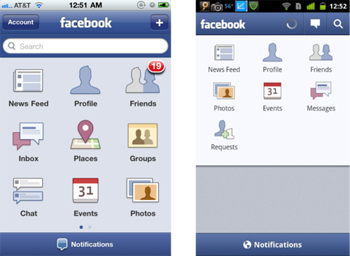
\includegraphics[scale=.5]{iphone_android_facebook_ui.png}
\caption{\label{facebook_android_ios}A side-by-side view of the Facebook application for iPhone (left) and Android (right).}
\end{center}
\end{figure}

The greatest of all our anticipated problems lies with the interface.  Between three different development teams, iOS, Web, and Android, there are fundamentally different technologies behind each team's interface.  The iOS team seems intent on using the Cocoa API for their application, a standard that is in almost no way compatible with Java used for Androids.  Given our teams' basic understanding, it would seem as if this decision is preparing us for difficulties in matching the interfaces.  The Web development team, however, is using HTML5, an obvious choice for them.  Our use of the PhoneGap technology readily aligns us with their design and will allow for a unified feel between the website and the Android application.  This cohesion is going to make collaboration between our two teams much easier, resulting in a more stable and appealing product.  Working with the iOS team will simply require a greater volume of communication and effort, but it is not impossible to make applications with similar interfaces on iOS and Android.  \textbf{Figure~\ref{facebook_android_ios}} illustrates how the \textit{Facebook} application for iPhone and Android makes use of a distinctly similar look across platforms.  Although the same application, it is obvious that each is running on a different platform.  A similar visual theme is important for brand recognition and keeping individuals familiar with all the features a company has to offer.  It will be important for us to make similarity in design an issue of quality rather than a convenience.

\section{Estimated Timeline}
Each of the following goals is to be completed by the specified date.  While we intend to meet each deadline, there are no guarantees in software development.
\begin{description}
\item \textbf{Monday the 26th of September}: Meet and put together all the parts of the initial plan – team name, list of members, members profiles, description of final project, key features in final project, list of tools that will be used, biggest challenges, and finally this schedule.

\item \textbf{Tuesday the 27th of September}: Turn in initial plan including all parts asked for in the assignment.

\item \textbf{Thursday the 29th of September}: Become extremely familiar with HTML5, JavaScript and Phonegap so
that we can begin coding known features designing an extensive class diagram.

\item \textbf{Thursday the 13th of October}: Draft an application capable of pushing and pulling data from the server, allow for testing speeds and any other issues the server may have with the constant push/pull of position data that this game will require.  Additionally: test the Websockets Pong demo available at \begin{verbatim}
https://github.com/german/pong
\end{verbatim}

\item \textbf{Thursday the 20th of October}: Be able to connect and receive data from Wii Remote, this will be our first prototype.  It should receive Wii Remote data and depending on the form convert it and send position data to the server. This will allow the server to test its functionality and game engine and allow the testing of
accelerometer accuracy for position.  This functionality depends primarily on the Wii Remote team's communication package.

\item \textbf{Thursday the 27th of October}: Test a working game engine that plays based off of position data given by Wii Remote accelerometer. At this point we will know what kind of data we will be receiving and can create a graphic that moves paddle and ball position based on data sent from the server. Around this time,
documentation for the Android SDK and ADT should be finished, allowing programmers in other groups
or on GitHub to install everything, look at our code, and make improvements or suggestions.

\item \textbf{Thursday the 3rd of November}: We will start finishing other key features such as matching system and stats tracker, begin work on JavaScript, CSS3, and HTML5 documentation. At this point someone who has
installed the application should be able to play. This is a fully functional prototype of the application.

\item \textbf{Thursday the 10th of November }: Proceed with full testing and the addition of any secondary features. This includes trying everything we can that may break the application and
compatibility testing with the iPhone. This would be the time to finish up all other documentation and
begin working on install documentation. At this point, assuming everything follows schedule, we should
have a nearly finished and working human Pong game.
\end{description}






















\end{document}
